\documentclass{article} % Класс печатного документа

% для поддержки русского языка
\usepackage[T2A]{fontenc} % поддержка специальных русских символов
\usepackage[utf8]{inputenc} % Кодировка исходного текста - utf8
\usepackage[english,russian]{babel} % Поддержка языка - русского с английским
\usepackage{indentfirst} % Отступ в первом абзаце

\usepackage{hyperref} % Для вставки гиперссылок
% \usepackage{listings} % Для вставки кусков кода
\usepackage{graphicx} % Вставка изображений
\usepackage{subfig} % Изображения друг напротив друга
\usepackage{float} % Для точного позиционирования картинок

% Default fixed font does not support bold face
\DeclareFixedFont{\ttb}{T1}{txtt}{bx}{n}{12} % for bold
\DeclareFixedFont{\ttm}{T1}{txtt}{m}{n}{12}  % for normal

% Custom colors
\usepackage{color}
\definecolor{deepblue}{rgb}{0,0,0.5}
\definecolor{deepred}{rgb}{0.6,0,0}
\definecolor{deepgreen}{rgb}{0,0.5,0}

\usepackage{listings}

% Python style for highlighting
\newcommand\pythonstyle{\lstset{
    language=Python,
    basicstyle=\ttm,
    otherkeywords={self},             % Add keywords here
    keywordstyle=\color{deepblue},
    emph={MyClass,__init__},          % Custom highlighting
    emphstyle=\color{deepred},    % Custom highlighting style
    stringstyle=\color{deepgreen},
    frame=tb,                         % Any extra options here
    showstringspaces=false,           % 
    basicstyle=\small,                % уменьшить размер шрифта
    columns=flexible                  % чтобы при копировании не было пробелов везде
}}


% Python environment
\lstnewenvironment{python}[1][]
{
\pythonstyle
\lstset{#1}
}
{}

% Python for external files
\newcommand\pythonexternal[2][]{{
\pythonstyle
\lstinputlisting[#1]{#2}}}

% Python for inline
\newcommand\pythoninline[1]{{\pythonstyle\lstinline!#1!}}

\makeatletter
\def\lst@outputspace{{\ifx\lst@bkgcolor\empty\color{white}\else\lst@bkgcolor\fi\lst@visiblespace}}
\makeatother
 % для красивого оформаления python кода

\title{Отчёт 5\protect\\
    Классификация.\\
    Метод деревьев классификации и регрессии\\
    (classification and regression trees - cart)} % Заголовок документа
\author{Свичкарев А.\,В.} % Автор документа
\date{\today} % Текущая дата

\begin{document} % Конец преамбулы, начало текста

\maketitle % Печатает заголовок, список авторов и дату

\section{Цель}
Изучить способы решения задач классификации данных с
применением метода CART

\section{Задание №1}
Написать программу построения модели классификации данных методом CART и
визуализации дерева решений. Сравнить полное дерево с деревом, полученным после его
сокращения (pruning) с параметром 0.1.
\bigskip

Реализация взята из Приложения.
Но в исходном примере присутствует ошибка в функции вывода дерева в консоль.
\bigskip

Реализация алгоритма построения деревьев,
их вывода и предсказания (файл \verb$treeclassification.py$):
\pythonexternal{../treeclassification.py}

\clearpage
Запускающий модуль (файл \verb$exercise1.py$):
\pythonexternal{../exercise1.py}
\bigskip

Вывод программы:
\lstinputlisting{./ex1_output.txt}

% \clearpage
% \section{Задание №2}
% Написать программу классификации данных методом k-ближайших соседей при
% нескольких различных значениях k с использованием обучающей выборки из предыдущей
% задачи.
% \bigskip
%
% Запускающий модуль выглядит так (файл \verb$exercise2.py$):
% \pythonexternal{../exercise2.py}
% \bigskip
%
% Вывод программы:
% \lstinputlisting{../output_exercise2.txt}
%
% \clearpage
% \section{Задание №3}
% Написать программу классификации данных методом k-ближайших соседей для данных из
% практических работ №1-№3. Для обучения использовать результаты кластеризации
% данных. Затем в качестве обучающей выборки использовать часть данных (варьируя объем
% в интервале [100\%-50\%]) с номером класса из задачи кластеризации. Применить метод
% классификации к оставшимся данным – включив их в тестовую выборку.
% \bigskip
%
% Была взята генерируемые двумерные выборки из нормального распределения
% из 1 задания.
% Пример генерации:
%
% \noindent\makebox[\textwidth]{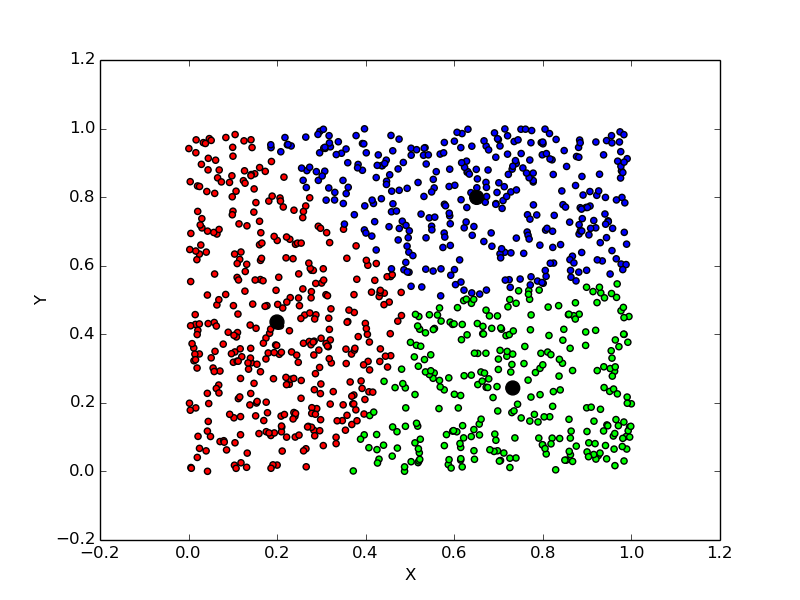
\includegraphics[width=0.7\paperwidth]{Figure_1}}
%
% Запускающий модуль выглядит так (файл \verb$exercise3.py$):
% \pythonexternal{../exercise3.py}
% \bigskip
%
% Вывод программы:
% \lstinputlisting{../output_exercise3.txt}
% \bigskip
%
% Как видно при сильно сгруппированных
% пространственно выборках,
% метод ближайших соседей даёт лучшие результаты.

\section{Пояснение}
Исходный код доступен по ссылке:
\href{https://github.com/SvichkarevAnatoly/Course-Python-Bioinformatics/tree/master/semester2/task5}
{github.com}

\end{document} % Конец документа
